\documentclass[border=4pt]{standalone}
\usepackage{amsmath,amssymb}
\usepackage{tikz}
\usetikzlibrary{shadows,decorations.pathreplacing,calc}
\begin{document}
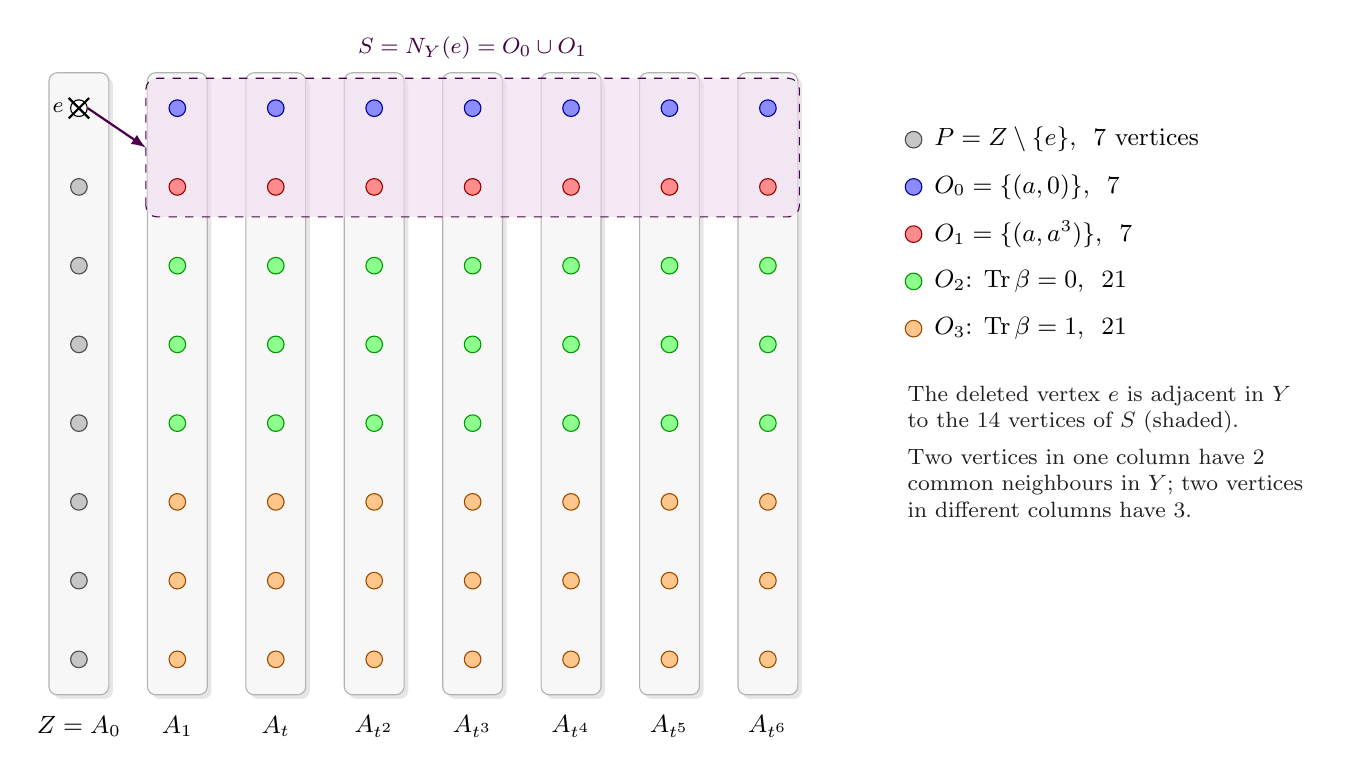
\begin{tikzpicture}[
  v/.style={circle,draw=#1!60!black,fill=#1!45,inner sep=0pt,minimum size=6pt},
  col/.style={draw=gray!60,fill=gray!6,rounded corners=3pt,
              drop shadow={opacity=0.2,shadow xshift=1.5pt,shadow yshift=-1.5pt}},
  lab/.style={font=\small},
  note/.style={font=\footnotesize,gray!25!black}]
  % columns: the eight cosets of the centre Z
  \foreach \j/\name in {0/{Z=A_0},1/{A_{1}},2/{A_{t}},3/{A_{t^2}},4/{A_{t^3}},5/{A_{t^4}},6/{A_{t^5}},7/{A_{t^6}}} {
    \pgfmathsetmacro{\x}{1.25*\j}
    \draw[col] (\x-0.38,-0.45) rectangle (\x+0.38,7.45);
    \node[lab] at (\x,-0.85) {$\name$};
  }
  % the neighbours of e form S = O_0 u O_1: the top two rows of A_1, ..., A_{t^6}
  \fill[violet!14,fill opacity=0.6,rounded corners=4pt] (0.85,5.62) rectangle (9.15,7.38);
  \draw[violet!60!black,dashed,rounded corners=4pt] (0.85,5.62) rectangle (9.15,7.38);
  \node[font=\footnotesize,violet!50!black,anchor=south] at (5,7.5) {$S=N_Y(e)=O_0\cup O_1$};
  % the centre: e (deleted) and P
  \node[circle,draw=black,fill=white,inner sep=0pt,minimum size=6pt] (e) at (0,7) {};
  \draw[thick] ($(e)+(-0.13,-0.13)$) -- ($(e)+(0.13,0.13)$) ($(e)+(-0.13,0.13)$) -- ($(e)+(0.13,-0.13)$);
  \node[font=\footnotesize,left=2pt] at (e) {$e$};
  \draw[violet!60!black,thick,-latex] (e.east) -- (0.85,6.5);
  \foreach \i in {0,...,6} { \node[v=gray] at (0,\i) {}; }
  % the other cosets: one vertex of O_0, one of O_1, three of O_2, three of O_3
  \foreach \j in {1,...,7} {
    \pgfmathsetmacro{\x}{1.25*\j}
    \node[v=blue]   (s0\j) at (\x,7) {};
    \node[v=red]    (s1\j) at (\x,6) {};
    \foreach \i in {3,4,5} { \node[v=green] at (\x,\i) {}; }
    \foreach \i in {0,1,2} { \node[v=orange] at (\x,\i) {}; }
  }
  % legend
  \begin{scope}[shift={(10.6,6.6)}]
    \node[v=gray]   at (0,0)    {}; \node[lab,right=4pt] at (0,0)    {$P=Z\setminus\{e\}$, \ $7$ vertices};
    \node[v=blue]   at (0,-0.6) {}; \node[lab,right=4pt] at (0,-0.6) {$O_0=\{(a,0)\}$, \ $7$};
    \node[v=red]    at (0,-1.2) {}; \node[lab,right=4pt] at (0,-1.2) {$O_1=\{(a,a^3)\}$, \ $7$};
    \node[v=green]  at (0,-1.8) {}; \node[lab,right=4pt] at (0,-1.8) {$O_2$: $\operatorname{Tr}\beta=0$, \ $21$};
    \node[v=orange] at (0,-2.4) {}; \node[lab,right=4pt] at (0,-2.4) {$O_3$: $\operatorname{Tr}\beta=1$, \ $21$};
    \node[note,anchor=north west,text width=5.2cm,align=left] at (-0.2,-3.0)
      {The deleted vertex $e$ is adjacent in $Y$ to the $14$ vertices of $S$ (shaded).\\[4pt]
       Two vertices in one column have $2$ common neighbours in $Y$; two vertices in different columns have $3$.};
  \end{scope}
\end{tikzpicture}
\end{document}
